%!TEX root = main.tex

\section{Motivation and Framework}
In this section, we setup the context by introducing how today's web backends optimize QoE.
Then we show the observation that there is a great heterogeneity in the sensitivity of QoE to backend delay across requests, which inspires a new QoE-driven approach to web backend design.
%Then we give the empirical observation that there is great heterogeneity in the sensitivity of QoE to backend delay across requests, which inspires new opportunities to improve the QoE/resource tradeoffs of the web service backends without adding new resources. 
%Finally, we give a framework that contrasts today's approach with our proposed one.

\subsection{Today's approach}
% - Architecture of web service
%\mypara{A canonical architecture} 
\begin{wrapfigure}{r}{0.43\linewidth}
	\centering
	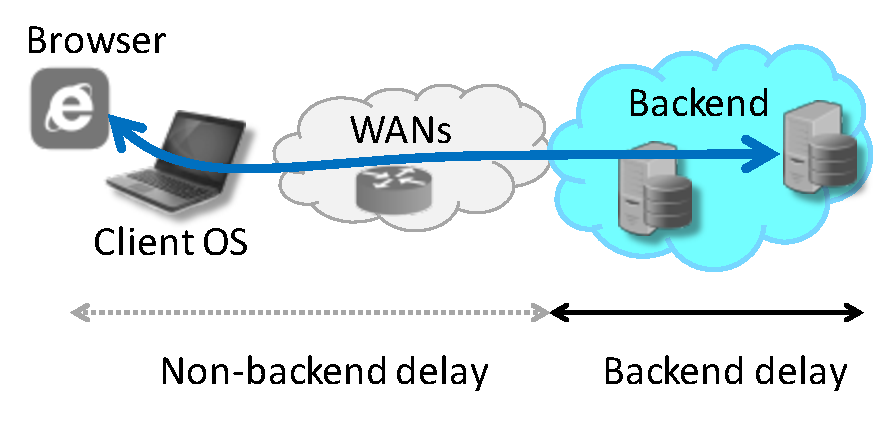
\includegraphics[width=0.95\textwidth]{figs/background.pdf}
	\caption{High-level architecture of today's web service and the lifecycle of a web request.}
	\label{fig:background}
\end{wrapfigure}
Figure~\ref{fig:background} depicts the high-level architecture of large-scale web services, and the lifecycle of a web request.
When a web request is issued by a user (\eg loading of a front page), it typically involves three components---client software, wide-area networks (WANs), and the backend---before the response is showed to the user.
The delay of each component contributes to the end-to-end delay and thus the user-perceived QoE (assuming the requested data is not cached locally by the client/ISP, etc). 
%In today's federated Internet architecture, the web service provider typically only has the control over the backend-induced delay. 
%Note that although client-side browsers/apps are developed by web service providers, the client-side delay is largely decided by how OS share resources among applications. 
A web service backend can be viewed as solving a resource sharing problem: optimizing the performance of many requests using a limited amount of resources. 
With the web service providers only controling the backend and the backend-induced delay\footnote{Although client-side browsers/apps are developed by web service providers, the client-side delay is largely decided by how OS share resources among applications.}, they seek to minimize the backend delay. 


% - Optimization metrics of each components: not QoE specific!
%\mypara{Today's approach}

While they measure the backend delay in different forms, today's backend systems share a common assumption (though often made implicitly) that the backend delay has the {\em same effect} on any request; \eg a delay of 20ms reading data from a database degrades the QoE by the same amount for any request . 
Under this assumption, it is sensible to measure performance by mean or percentiles (\eg 99$^\textrm{th}$ percentile) of backend delay or percentage of requests whose delays exceed some threshold (\eg service-level agreement).

Here, we only consider requests of the same application-level type, \eg content genre, user subscription type.
Note that even under the assumption that backend delay impact QoE in the same way for any request, requests can still be treated differently. For instance, in deadline-driven congestion control~\cite{??}, when congestion occurs, a small number of randomly picked flows might be delayed so that most flows can meet the deadline of flow completion time. 

\subsection{Key insight: Heterogeneity of QoE sensitivity}
%\jc{throw in some concrete improvement numbers}

Contrary to the assumption of backend delay having equal impact on QoE for any request, our key observation is that 
{\em the sensitivity of QoE to the backend delay varies across requests.}
%Our key observation is that the impact of backend delay on the QoE of a request actually depends on how much non-backend delay (Figure~\ref{fig:background}) the request experiences, including the client-induced and WAN-induced delays. 
%In other words, {\em the sensitivity of QoE to the backend delay varies across requests.} 
%\mypara{Why QoE sensitivity varies}

\begin{wrapfigure}{r}{0.5\linewidth}
	\centering
	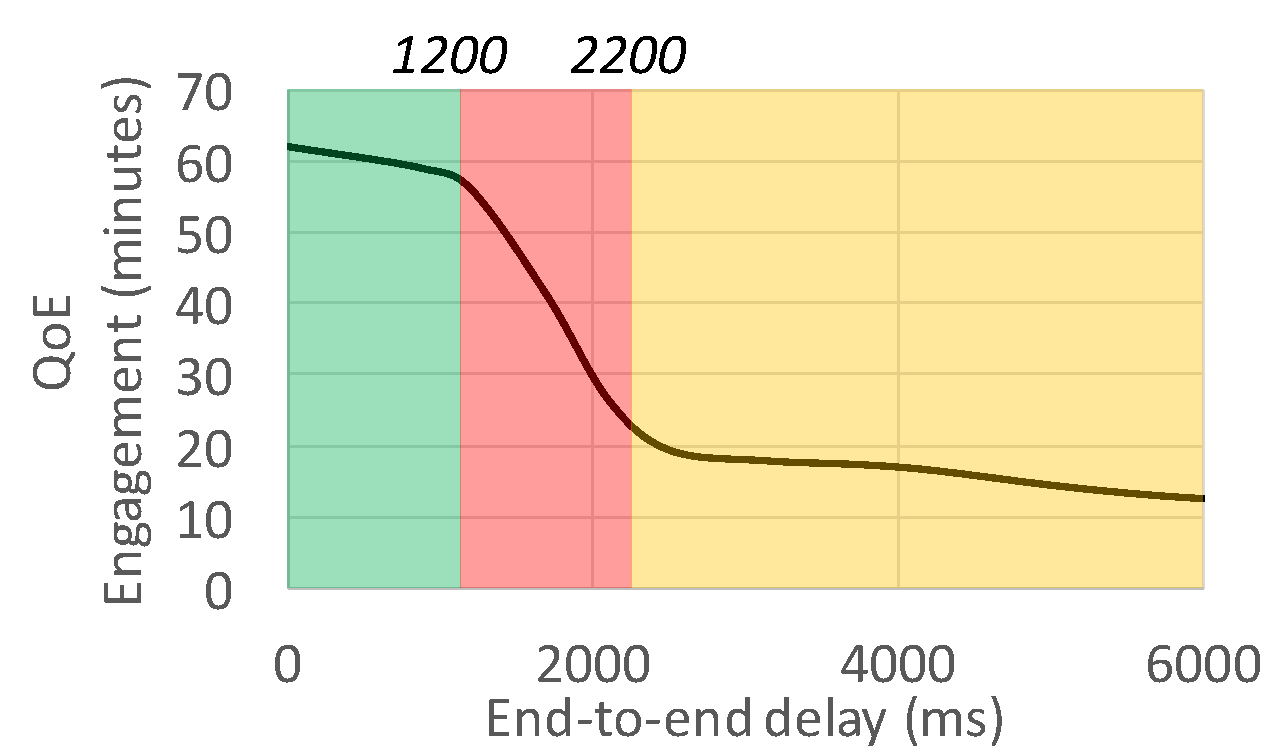
\includegraphics[width=0.95\textwidth]{figs/qoe-curve.pdf}
	\caption{QoE curve showing the relationship between QoE and the end-to-end delay of a request.}
	\label{fig:qoe-curve}
\end{wrapfigure}
Figure~\ref{fig:qoe-curve} illustrates the intuition behind this observation using a dataset of \fillme web requests. The requests are from one of the Alex top-50 webpage, thus avoiding the impact of content on QoE. The requests were recorded in a period of 24 hours from users in \fillme countries, thus representing a decent coverage over space and temporal diversity.
The figure shows the relationship between QoE and the end-to-end delay of a request, which we refer to as the {\em QoE curve}.
%It is based on \fillme requests to a particular page (\fillme), thus avoiding the impact of content on QoE. 
For each request, we use the duration between the request is completed and the user leaves the web site domain (subsequent clicks from the page are counted as part of the session too) as the QoE metric. 
User engagement, like session duration, is typically used as subjective way of measuring QoE~\cite{engagement}.
The page load time is calculated by subtracting when the page is completely loaded by when the request is issued. 

The QoE curve is non-linear (sigmoid-shaped).\footnote{This curve may vary with the nature of the web sites and the requests (\eg QoE in general is less sensitive to delay when the user really needs to see the content of the page than when the website tries to entice users to do something), yet the sigmoid-like shape remains.}
This means that same amount of increase of page load time will have different effect on the QoE, depending on the position of starting point on the curve.
It can be intuitively explained. 
Users are not sensitive to a small change in delay when the overall delay is very short (below roughly 1200ms), because users typically gets annoyed by the delay only when it exceeds some threshold, or too long (above 2200ms), because the user has mostly tired of waiting. Only when the total delay is in the middle (roughly between 1200ms and 2200ms) can some change make a significant difference. 
%Secondly, we observe that the non-backend delays (client- and WAN-induced delays) of the requests are not concentrated in certain segment of the curve; rather, they spread out over the curve.
%In our dataset, we found \fillme\% requests have non-backend delay are below 1200ms, \fillme\% between 1200ms and 2200ms, and \fillme\% above 2200ms. 
%Combining this observation with the non-linear relationship between delay and QoE, we see that the sensitivity of QoE to the backend delay varies among requests. 


%\myparaq{What is new}
Indeed, we are not the first to observe the heterogeneity in non-backend delay across requests~\cite{timeciard,dqbarge} and the non-linear delay-QoE relationship~\cite{d3tcp, mun chiang's work}---in fact, the assumption that application flows have deadline utility function can be viewed as a simplification of the non-linear delay-QoE relationship.
What is new is their corollary that requests have different QoE sensitivity to backend delay, which, as we will see next, has a profound implication on QoE optimization. %how resource consumption and QoE optimization should be balanced.
%if the backend can add a total backend delay of $\delta=\delta_a+\delta_b$ to the two requests ($A$ gets $\delta_a$ and $B$ gets $\delta_b$), traditional methods will give both $A$ and $B$ a delay of $\delta/2$, whereas better QoE can be achieved by letting $\delta_a<\delta_b$. 
%We will give more concrete examles in \S\ref{sec:design}.

\subsection{New opportunities}
At a high level, the heterogeneous QoE sensitivity means that rathter than treating all requests as having equal sensitivity to the same amount of backend resources, the backend should instead allocate idle resources to requests that are more sensitive to backend delay.
To see it in action, suppose that request $A$ with non-backend delay $x_a$ is more sensitive to the backend delay (the red area of Figure~\ref{fig:qoe-curve}) than request $B$ with non-backend delay $x_b$ (the green or yellow area of Figure~\ref{fig:qoe-curve}). Now, if the backend resource allocation is such that one of them will get a backend delay of $\delta_1$ and the other one $\delta_2$, $\delta_1>\delta_2$. A QoE-agnostic method may make a random decision (\eg 50\% probability $A$ will get an end-to-end delay of $x_a+\delta_1$), but a QoE-driven method should instead assign the smaller backend delay $\delta_2$ to $A$, because $A$ is more sensitive to backend delay.

This simple example illustrates that the opportunities of QoE-driven depend on two factors.
First, both requests whose QoE is sensitive to the backend and those whose QoE is not must be present. As shown in Figure~\ref{fig:qoe-curve}, we found 41.5\% requests have QoE that is sensitive to the backend delay (red region between 1200ms and 2200ms), and the rest (29.8\% in the green region and 28.7\% in the yellow region) have QoE that is not as sensitive to the backend delay.
Second, requests should have different backend delay, which distributed systems naturally have for a number of reasons, \eg jobs in a queue will naturally have different waiting time, or replicas will naturally have different performance since they have different load.

%\jc{add inefficiency of non-QoE-aware approaches: 
%resources wasted, packing qoe-sensitive users with non-sensitive users}

\subsection{Framework}
\label{subsec:framework}
\begin{wrapfigure}{r}{0.45\linewidth}
	\centering
	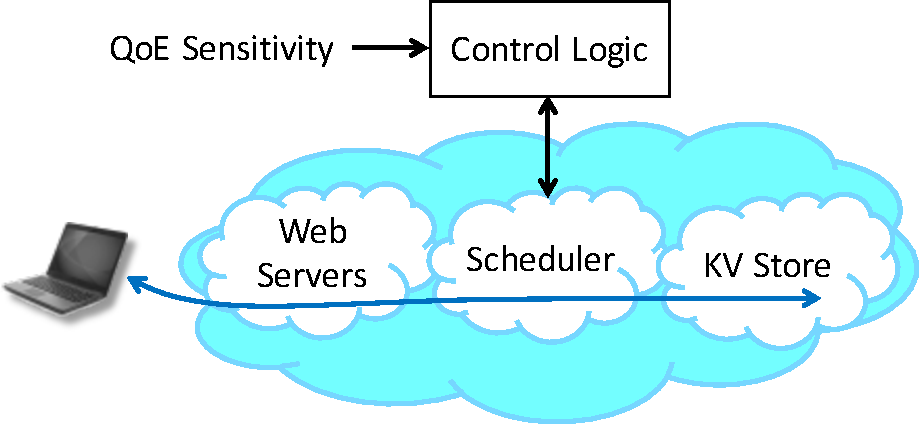
\includegraphics[width=0.95\textwidth]{figs/framework.pdf}
	\caption{}
	\label{fig:framework}
\end{wrapfigure}
Next we present a high-level framework (Figure~\ref{fig:framework}) of transforming today's web service backend with QoE-aware optimization.
% shows a conceptual view of a QoE-aware web service backend. 
A typical web service backend has multiple subsystems, \eg messaging system, distributed database, inter-datacenter networks, and any delay caused by any subsystem will contribute to the backend delay of a request.
Although these subsystems are owned by the same organization, today there is little orchestration across these subsystems to jointly optimize for each request. 
It is beyond our scope to discuss the cost of separating these subsystems. 



This proposal takes a pragmatic stance. 
We optimize each individual subsystem by proposing minimal necessary changes in its existing ``control logic''.
A control logic can be implemented in different forms---\eg scheduling logic, resource allocation logic, congestion control sending rate, but it essentially share the limited resource among many requests.
\begin{packeditemize}
    \item The control logic of a QoE-aware subsystem takes in as part of its input the QoE sensitivity of any incoming request---an estimate on its non-backend and the corresponding position on the QoE-latency curve. 
    We envision different ways in which this information would be provided; \eg through a service that predicts the non-backend delay of a new request by profiling the non-backend delay of similar history requests, or adding a field in the request for any subsystem to tag the time it leaves each subsystem. (More discussion in \S\ref{sec:arch}.)
    \item Then, the control logic needs to be updated so that it can utilize the discrepancy of QoE sensitivity among requests to strike better QoE/resource tradeoffs (\ie the benefits we discussed in \S\ref{subsec:opportunities}).
    The contrast between the proposed QoE-aware control logic and traditional control logic can be explained as following: 
    For each request $r$ in a set of requests $R$, let $t_{r}^{(nb)}$ denote the non-backend delay, and $t_{r}^{(b)}$ the backend delay, and $Q(t)$ the QoE of the total backend and non-backend delay $t$.
    Traditional logic seeks to minimize average backend delay, \ie
    \begin{align}
        & \min \sum_{r\in R} t_{r}^{(backend)} \label{eq:old}
    \end{align}
    whereas, QoE-aware logic seeks to minimize average degradation of QoE, \ie
    \begin{align}
        & \min \sum_{r\in R} Q\left(t_{r}^{(nonbackend)}\right)-Q\left(t_{r}^{(nonbackend)}+t_{r}^{(backend)}\right) \label{eq:new}
    \end{align}
\end{packeditemize}




\section{Quantifying Potential Benefits in the Wild}
\begin{task}
We will carry out measurement studies to quantify various benefits---in QoE and resource---of a QoE-aware web service backend.
\end{task}

%The heterogeneity of QoE sensitivity across requests opens up many new opportunities to strike better resource/QoE tradoffs. 
In this section, we provide a taxonomy to categorize various possibilities of using the heterogeneous QoE sensitivity to improve the web service backend.%, and show simple-yet-realistic motivating examples to highlight two concrete use cases.

\subsection{A taxonomy of improvement}

%\mypara{Benefits}
We categorize the performance advantages of a QoE-driven backend over today's backend systems in four types:

\mypara{Improving QoE} 
First and foremost, a QoE-driven backend can achieve better QoE than a traditional one, by allocating resources in a way that more explicitly optimizes the total QoE. 
Here, we use a simple trace-driven simulation to quantify this potential improvement. 
Take Figure~\ref{fig:}
%In contrast to today's web backends which focus on the mean (or percentiles) of backend delay, we argue that they should instead {\em minimize the impact of backend delay on QoE}, so more resources (\eg higher priority) should be given to requests whose QoE is more sensitive to the backend delay. 
    
\mypara{Mitigating the impact of performance outliers} 
A common challenge of web service backends is how to trim the performance outliers---requests that experience excessively long backend delay, \eg due to server garbage collections. 
Rather than trying to eliminate outliers, the QoE sensitivity offers a new approach to {\em reduce the degradation on QoE due to outliers}.
Then instead of spreading requests evenly across servers, we can profile the performance of servers and predict the servers that are likely to have outliers~\cite{ganesh's trimming}, and assign requests with less QoE sensitivity to these servers, and keep requests with higher QoE sensitivity away from these servers. 
    
\mypara{Resource savings}
Similarly, one can reduce resource consumption, and possibly save energy, by spending less resources to optimize requests of lower QoE sensitivity. For instance, this can be done by deprioritizing the low QoE-sensitivity requests or sending them to servers with higher load, 
Doing so may be seen as unfair, but as we will discuss in \S\ref{sec:arch}, this can still be fair in the sense that each request gets an equal treatment (degradation) on the QoE.
    
\mypara{Cost-efficient explorations}
Finally, to cope with dynamic resource availability, backend systems (\eg CDN) maintain the visibility of many decisions (\eg edge clusters), by sending a fraction of request to randomly explore suboptimal decisions or injecting active probing traffic.
Neither approach is ideal. 
We take a different approach---one can use the requests of low QoE sensitivity to probe the suboptimal decisions, as long as the QoE degradation does not exceed that of sending a request of high QoE sensitivity to the optimal decision.
This way, we can maintain visibility with less impact on QoE.
%\end{packeditemize}
Note that these benefits can be realized without expensive adding more hardware or changing software stack, and can be done incrementally (they have no inter-dependency).

\mypara{Use cases}
These benefits can manifest themselves in many subsystems (Figure~\ref{??}) throughout a web service backend.
\begin{packeditemize}
\item {\em Scheduling:}

\item {\em Replica selection:} 

\item {\em Congestion control:}

\end{packeditemize}

\subsection{Proposed research}

- Quantifying the QoE-delay curve in the wild

- Quantifying the heterogeneity of QoE sensitivity

- Impact of QoE-aware logic on QoE (maybe delay is too small to be noticed anyway)





\section{Designing QoE-Aware Web Service Backend}
\label{sec:design}

\begin{task}
We will develop new scheduling and replica selection policies that leverage the heterogeneity of QoE sensitivity across requests to improve user-perceived QoE.
\end{task}

\subsection{Why new algorithms are needed?}

\mypara{Message scheduling}
% - fifo and etc don't work
To show the need of a new policy for QoE-driven  scheduling, we consider a simple example (shown in Figure~\ref{??} ) in which there are three identical requests (\ie they are of the same priority) in the queue but they have different non-queuing delays.
We compare three policies: 
(1) FIFO, which is the default policy for equal-priority requests.
(2) Earliest-Deadline-First (EDF), which uses a fixed deadline on the sum of queuing delay and non-queuing delay and prioritizes requests whose non-queuing delay is closest to the deadline, and 
(3) the optimal scheduling policy (OPT) that maximizes average QoE.
We assume that the page load time of a request is the sum of the non-queuing delay and the queuing delay (that is, the number of jobs ahead of it times the per-request processing delay).
Figure~\ref{??}  shows the outcome of running each policy. 
We can see that OPT outperforms FIFO, because it is agnostic to non-queuing delay
OPT also outperforms EDF with various deadlines, even though it somehow takes the non-queuing delay into account (by imposing a deadline on the total of queuing and non-queuing delay).
This is because how close a request's non-queuing delay is to the deadline is {\em still} agnostic to the sensitivity of QoE to the queuing delay. 
Remember in Figure~\ref{??}, the QoE sensitivity does not grow monotonically to the non-backenc(queuing) delay. 

\mypara{Web server replica selection}
% - example of tails
Large-scale distributed systems are susceptible to {\em performance outliers} on some replicas---\eg exceptionally long processing time on some requests due to CPU contention, software garbege collection, etc. 
Despite much effort devoted to eliminate performance outliers, they are still prevalent, resulting in bad tail (\eg 99$^\textrm{th}$ percentile) performance even if the mean/median performance is good.
Our first idea is that rather than cutting the performance outliers, we show that QoE-aware replica selection algorithm can {\em contain} the negative impact of performance outliers on user-perceived QoE.

Consider a system with two replicas, as in Figure~\ref{??}. 
Both replicas have the same load-performance profile that as load (number of requests received per second) goes up, the 99$^\textrm{th}$ percentile delay increases sharply, though the mean performance has only mild increase. 
This illustrative setting is simplified but in consistent with the load-performance profile in real datacenters~\cite{??}.
Suppose that the workload is \fillme requests per second, that the requests have same QoE-delay curve, and their non-backend delays follow the distribution show in the figure.
We compare two traditional replica selection policies---load balancing policy that strives to put even load, latency-aware policy~\cite{c3,cassandra,etc} that optimizes for Eq.~\ref{eq:old}---with an optimal policy that optimizes for Eq.~\ref{eq:new}.
We see that the optimal solution achieves better tail QoE than both baselines. 
Both load balancing policy and latency-aware put even load to the replicas, which make both equally overloaded, causing long tail delay and bad tail QoE.
In contrast, the optimal policy diliberately puts more requests on one than another, but does so by letting QoE-sensitive requests use the lighter-loaded replica and letting QoE-insensitive requests use the slightly more loaded replica. 

\subsection{Why challenging?}
The new QoE-aware scheduling policy should be {\em near-optimal} (\ie achieve QoE close to the optimal scheduling outcomes) and {\em efficient} (\ie constant decision time on each incoming request).
To see why it is challenging to meet both requirements simultaneously, let us consider two baselines.
On one hand, standard approximating\footnote{Unfortunately, optimzing a non-contex curve objective function, as in our case, requires running complex algorithms, whose runtime increases super-linearly with the number of variables~\cite{??}.} algorithms (\eg~\cite{??}) often requires non-constant overhead to compute the scheduling order of each request. 
On the other hand, fast scheduling algorithms can be suboptimal. 
For instance, one efficient scheduling algorithm is to give each request a priority that is proportional to the {\em slope} of its non-queuing delay on the QoE-delay curve. 
This makes sense, because if the request were to stay in the queue for a (short) fixed amount of queuing delay, this slop indicates exactly how much QoE degradation will be caused by the queuing delay, and the decision runtime is constant for each request.
However, the queuing delay does vary among requests as well as over time (as it might be pre-emptived by future requests), and the resulting QoE might suffer.
If the queuing delay is non-trivial, the slope of a request's non-queuing delay can be both an overestimate or underestimate of the acutal QoE sensitivity of a request. 
In Figure~\ref{??}, for instance, if the queuing delay is 200ms, a request with 1100ms non-queuing delay will be believed as insensitive to the queuing delay, while after 200ms queuing, it actually will see significant drop in QoE. 

Moreover, the new scheduling policy has to be {\em amenable} to the implementation of existing message brokers. 
For instance, in RabbitMQ, once a request is pushed to a FIFO queue associated with some priority, and cannot be easily changed to another FIFO queue. 
That means, the related ordering of two requests cannot be changed once they are scheduled.
For instance, the aforementioned slope-based scheduling algorithm cannot be easily fixed by re-assigning a priority that reflects the slope after the amount of queuing delay.
(Note this does not preclude the possibility of preemption by a future request if we assign it with a high priority.)

\subsection{Proposed research}
We propose to develop new scheduling policies that leverage the heterogeneity of QoE sensitivity across requests to improve user-perceived QoE. 
One potential idea is to rely on the fact that the number of requests and the distribution of their non-queuing delay is relatively stable at a timescale of several seconds. 
Thus, we can periodically recalculate the priority of a request with certain non-queuing delay by assuming that future requests will be drawn from certain distribution.
Then, the scheduling problem can save this mapping in a table, and determine the priority of any new request by looking-up the table. 




\section{A New Architecture, a New Way of Thinking}
\label{sec:arch}

This section focuses on two basic architectural questions behind QoE-driven backend---how to make web backend know of the QoE sensitivity and how should fairness be defined in our context.

\subsection{How to make web backend aware of QoE sensitivity?}
\begin{task}
We will explore new architectural component of web backend, including tracing infrastructure and QoE prediction models, to estimate the QoE sensitivity of requests in real-time.
\end{task}

\mypara{Estimating non-backend delay}
Making web backend aware of a request's QoE sensitivity is difficult in today's federated Internet architecture with the web backend system only having the visibility of the delay within its own system (Figure~\ref{??}), while QoE, defined by either subjective user satisfaction or end-to-end response time, is only observable by the clients themselves. 
We envision that the QoE-delay curve, \ie relationship between end-to-end delay and QoE, should be profiled offline (for each content/application), because it is not expected to change frequently.
If the backend knows the non-backend delay of any incoming request, it would then be able to derive the QoE sensitivity of the request from the QoE-delay curve. 
We envision two basic approaches to measure the non-backend delay of a new request. 
\begin{packeditemize}
\item {\em History-based:}
One approach is to use the non-backend delay of history requests to build a prediction model that given any new request, can predict the non-backend delay. Once a request is completed, the web site or content provider will know its end-to-end delay (\eg via client-side instrumentation), and by matching the end-to-end delay with with get the non-backend delay with the backend delay measured by the backend, we can get the non-backend delay of this history request.

\item {\em Tracing-based:}
Another approach is directly estimate the non-backend delay of a request using the tracing infrastructure on the client and backend to directly measure the delay between when the client issues the request and when the backend receives it, \ie the ``incoming half'' of the non-backend delay. Prior work has found that this incoming half of the non-backend delay is indicative of (though not equal to) the ``outgoing'' half of the non-backend delay~\cite{timecard}.
\end{packeditemize}
Note that the two approaches represent a tradeoff---the history-based approach requires no additional real-time tracing of a new request and thus less intrusive to the existing system, whereas the tracing-based approach is more intrusive but might be more accurate as it directly measures the request under consideration.

\mypara{What pieces in today's systems can be used}
In fact, the tracing infrastructure, similar to what is needed for the tracing-based approach, is already available in several large-scale web service infrastructures. Facebook has introduced such a tracing system~\cite{mysterymachine}. Microsoft has a similar internal tracing system that keeps track of several key timestamps of a request (\eg when is issued by client, received by the edge web server, received and processed by a backend database)~\cite{sid's paper}.

\mypara{Proposed research}
%- Cross-subsystem tracing and predicting non-backend delay
While both approaches sound promising, we found that they may not meet the requirement of estimating QoE sensitivity of requests in real-time. 
These tracing systems and QoE recording systems are mainly built for {\em offline} diagnosis, rather than online inference. As a result, these timestamps are often recorded by individual subsytems in a distributed fashion, but only collected to a central place that can be queried every several minutes or even hours. 
To address this problem requires a better solution. 
One possibility is to make these tracing information (\eg timestamps of the past events of a request) ``in-band'' as part of the request itself. This may require changes in the message format or client-facing interfaces, but will make these tracing information instantly available when the backend recives the request.

\subsection{How should fairness be defined?}
\begin{task}
We will investigate the ``price of fairness'', \ie loss in QoE in exchange for more fairness, and how to define fairness that is robust to actions of other systems.
\end{task}

One evident downside of QoE-driven control policies is the seemingly unfair treatment of priorizing requests with higher QoE sensitivity over others, even though these requests are of the same nature (same application, same content, etc).

\mypara{This might be fair after all}
At first glance, giving more resources to one request than another, just because one request spends less (or more) time over the WAN, does not seem fair.
However, if we take the ``utility'' of these resource into account, such behavior could be viewed as perfectly fair under some circumtances.
More specifically, from the perspective a client, what matters is not how much resource her request is being process with; what matters is how much {\em QoE degradation} a particular resource allocation causes.
To use the  terminology  introduced in \S\ref{subsec:framework}, we can define fairness based on standard fairness index (\eg Jain's index~\cite{??}) over the QoE degradation, \ie $Q\left(t_{r}^{(nonbackend)}\right)-Q\left(t_{r}^{(nonbackend)}+t_{r}^{(backend)}\right)$, among requests $r\in R$.
More importantly, achieving this notion fairness can be directly incorporate in the solving the Eq.~\ref{eq:new} as a constraint.
%To use the terminology used in \S\ref{subsec:framework}, we can define a max-min fairness as
%\begin{align}
%& \min\max_{r\in R}Q(t_{r}^{(nb)})-Q(t_{r}^{(nb)}+t_{r}^{(b)}) \label{eq:fairness}
%\end{align}
%Under the Nash standard, a transfer of resources between two players is favorable and fair if the percentage increase in the utility of one player is larger than the percentage decrease in utility of the other player. 
%In our context, the Nash standard means that our resource allocation is favorable and fair, as long as the any transfer of resource will result in larger percentage of decrease in the QoE of one request than the percentage of increase in the QoE of another request.

%\mypara{Fairness under cross-entity settings}
%However, achieving fairness can be more difficult, if multiple subsystems (\eg message broker and web server selection) in web backend make QoE-driven decisions {\em independently} .
%Consider a backend of two consecutive subsystems $X$ and $Y$, \ie any request will go through $X$ and then $Y$ so that the backend delay is the sum of the two subsystems. 
%Now, suppose request $A$ has a greater non-backend delay than request $B$, which makes $A$ more sensitive to the backend delay than $B$. 
%So naturally, subsystem $X$ might process $A$ with greater backend delay than $B$. However, after considering this, 

\mypara{This can be taken advantage of}
However, achieving fairness can be tricky, if another system (\eg ISP) knows that the web backend allocates resources among request in the proposed way. In particular, the other system can trick the web backend into treating requests unfairly.
Consider a simple example where the end-to-end delay of a request is the delay of ISP $X$ and the delay of a web backend $Y$, and there  two requests $A$ and $B$.
Now, suppose ISP $X$ adds a small amount of delay to $B$ so that $B$'s QoE less sensitive to the backend delay than $A$. Following the principle of fair QoE degradation, backend $Y$ should treat $A$ and $B$ differently, giving more resource to $A$ than $B$. 
Note that $X$ would be able to do the same, if $Y$ defines fairness in a traditional sense (\ie with respect to backend delay, rather than QoE degradation).
While it seems oversimplified, this illustrates an underlying issue of QoE-driven web backend that by making the fairness metric and objective function linked with non-backend delay, we make the backend vulnerable to actions of other systems.

\mypara{Proposed research}
We will investigate the classic tradeoff between fairness and utility in the context of QoE-driven web backend. In particular, is it possible to solve Eq.~\ref{eq:new} in a near optimal fashion, as discussed in \S\ref{sec:design}, while maintaining, say max-min fairness, or there will be a price in fairness for better QoE.
In the meantime, we notice that by being QoE-agnostic, traditional web backends have already induced some unfairness in terms of user-perceived QoE. It would be helpful to compare our price of fairness with that of a traditional web backend, and see if we can still get sufficient QoE improvement by paying the same amount of price of fairness.

Finally, we will investigate how fairness should be defined so that we can avoid being negatively affected by other systems diliberately misleading our backend into treating requests unfairly. One potential solution is to monitor the delay of non-backend systems (\eg ISPs) of history requests in order to detect whether they add artificially add more delays; when they do, the backend then should stop inferring the requests' sensitivity by their actual non-backend delay; and instead assume the non-backend delay is at the normal level.


\section{Related Efforts}
Some earlier work also takes non-backend delay into account when optimizing cloud-based applications. 
Timecard~\cite{timecard} allows requests that have shorter network delay to wait longer for the web server to retrieve better ad content. 
DQBarge~\cite{dqbarge} similarly trades delay for better response quality by monitoring the progress of parallel subtasks and allowing faster subtasks to process longer to get better results without increasing the total response time.
Also relevant are works that dynamically predict the response-time service-level agreement of cloud applications~\cite{Rich Wolski}, which are driven by the same need to cope with the heterogeneity of non-backend delay across users and over time.
Our previous work EONA~\cite{eona} pioneers the idea of driving individual systems of the application ecosystem (including web service backend) by user-perceived QoE.
\jc{Difference to application-system joint optimization (\eg coflow)?}
However, none of these works show the benefits of QoE-awareness through the lens of resource/QoE tradeoffs. 

\jc{diff to QoE management. see wiki page.}


